%  template.tex for Biometrics papers
%
%  This file provides a template for Biometrics authors.  Use this
%  template as the starting point for creating your manuscript document.
%  See the file biomsample.tex for an example of a full-blown manuscript.

%  ALWAYS USE THE referee OPTION WITH PAPERS SUBMITTED TO BIOMETRICS!!!
%  You can see what your paper would look like typeset by removing
%  the referee option.  Because the typeset version will be in two
%  columns, however, some of your equations may be too long. DO NOT
%  use the \longequation option discussed in the user guide!!!  This option
%  is reserved ONLY for equations that are impossible to split across 
%  multiple lines; e.g., a very wide matrix.  Instead, type your equations 
%  so that they stay in one column and are split across several lines, 
%  as are almost all equations in the journal.  Use a recent version of the
%  journal as a guide. 
%  
\documentclass[useAMS,referee, usegraphicx]{biom}
%\documentclass[useAMS, usegraphicx]{biom}
%
%  If your system does not have the AMS fonts version 2.0 installed, then
%  remove the useAMS option.
%
%  useAMS allows you to obtain upright Greek characters.
%  e.g. \umu, \upi etc.  See the section on "Upright Greek characters" in
%  this guide for further information.
%
%  If you are using AMS 2.0 fonts, bold math letters/symbols are available
%  at a larger range of sizes for NFSS release 1 and 2 (using \boldmath or
%  preferably \bmath).
% 
%  Other options are described in the user guide. Here are a few:
% 
%  -  If you use Patrick Daly's natbib  to cross-reference your 
%     bibliography entries, use the usenatbib option
%
%  -  If you use \includegraphics (graphicx package) for importing graphics
%     into your figures, use the usegraphicx option
% 
%  If you wish to typeset the paper in Times font (if you do not have the
%  PostScript Type 1 Computer Modern fonts you will need to do this to get
%  smoother fonts in a PDF file) then uncomment the next line
%  \usepackage{Times}
\usepackage{amsmath}
\usepackage{graphicx}
\usepackage{url}

%%%%% PLACE YOUR OWN MACROS HERE %%%%%

\def\bSig\mathbf{\Sigma}
\newcommand{\VS}{V\&S}
\newcommand{\tr}{\mbox{tr}}

%  The rotating package allows you to have tables displayed in landscape
%  mode.  The rotating package is NOT included in this distribution, but
%  can be obtained from the CTAN archive.  USE OF LANDSCAPE TABLES IS
%  STRONGLY DISCOURAGED -- create landscape tables only as a last resort if
%  you see no other way to display the information.  If you do do this,
%  then you need the following command.

%\usepackage[figuresright]{rotating}

%%%%%%%%%%%%%%%%%%%%%%%%%%%%%%%%%%%%%%%%%%%%%%%%%%%%%%%%%%%%%%%%%%%%%

%  Here, place your title and author information.  Note that in 
%  use of the \author command, you create your own footnotes.  Follow
%  the examples below in creating your author and affiliation information.
%  Also consult a recent issue of the journal for examples of formatting.

\title[Mixture model detection functions]{Mixture models for distance sampling detection functions}

%  Here are examples of different configurations of author/affiliation
%  displays.  According to the Biometrics style, in some instances,
%  the convention is to have superscript *, **, etc footnotes to indicate 
%  which of multiple email addresses belong to which author.  In this case,
%  use the \email{ } command to produce the emails in the display.

%  In other cases, such as a single author or two authors from 
%  different institutions, there should be no footnoting.  Here, use
%  the \emailx{ } command instead. 

%  The examples below corrspond to almost every possible configuration
%  of authors and may be used as a guide.  For other configurations, consult
%  a recent issue of the the journal.

%  Single author -- USE \emailx{ } here so that no asterisk footnoting
%  for the email address will be produced.

%\author{John Author\emailx{email@address.edu} \\
%Department of Statistics, University of Warwick, Coventry CV4 7AL, U.K.}

%  Two authors from the same institution, with both emails -- use
%  \email{ } here to produce the asterisk footnoting for each email address

%\author{John Author$^{*}$\email{author@address.edu} and
%Kathy Authoress$^{**}$\email{email2@address.edu} \\
%Department of Statistics, University of Warwick, Coventry CV4 7AL, U.K.}

%  Exactly two authors from different institutions, with both emails  
%  USE \emailx{ } here so that no asterisk footnoting for the email address
%  is produced.

%\author
%{John Author\emailx{author@address.edu} \\
%Department of Statistics, University of Warwick, Coventry CV4 7AL, U.K. 
%\and
%Kathy Author\emailx{anotherauthor@address.edu} \\
%Department of Biostatistics, University of North Carolina at Chapel Hill, 
%Chapel Hill, North Carolina, U.S.A.}

%  Three or more authors from same institution with all emails displayed
%  and footnoted using asterisks -- use \email{ } 

%\author{John Author$^*$\email{author@address.edu}, 
%Jane Author$^{**}$\email{jane@address.edu}, and 
%Dick Author$^{***}$\email{dick@address.edu} \\
%Department of Statistics, University of Warwick, Coventry CV4 7AL, U.K}

%  Three or more authors from same institution with one corresponding email
%  displayed

\author{David L. Miller$^{*}$\email{dave@ninepointeightone.net}, 
Len Thomas\\
CREEM, University of St Andrews, The Observatory, Buchanan Gardens, St Andrews KY16 9LZ, Scotland}

%  Three or more authors, with at least two different institutions,
%  more than one email displayed 

%\author{John Author$^{1,*}$\email{author@address.edu}, 
%Kathy Author$^{2,**}$\email{anotherauthor@address.edu}, and 
%Wilma Flinstone$^{3,***}$\email{wilma@bedrock.edu} \\
%$^{1}$Department of Statistics, University of Warwick, Coventry CV4 7AL, U.K \\
%$^{2}$Department of Biostatistics, University of North Carolina at 
%Chapel Hill, Chapel Hill, North Carolina, U.S.A. \\
%$^{3}$Department of Geology, University of Bedrock, Bedrock, Kansas, U.S.A.}

%  Three or more authors with at least two different institutions and only
%  one email displayed

%\author{John Author$^{1,*}$\email{author@address.edu}, 
%Wilma Flinstone$^{2}$, and Barney Rubble$^{2}$ \\
%$^{1}$Department of Statistics, University of Warwick, Coventry CV4 7AL, U.K \\
%$^{2}$Department of Geology, University of Bedrock, Bedrock, Kansas, U.S.A.}


\begin{document}

%  This will produce the submission and review information that appears
%  right after the reference section.  Of course, it will be unknown when
%  you submit your paper, so you can either leave this out or put in 
%  sample dates (these will have no effect on the fate of your paper in the
%  review process!)

%\date{{\it Received October} 2007. {\it Revised February} 2008.  {\it Accepted March} 2008.}

%  These options will count the number of pages and provide volume
%  and date information in the upper left hand corner of the top of the 
%  first page as in published papers.  The \pagerange command will only
%  work if you place the command \label{firstpage} near the beginning
%  of the document and \label{lastpage} at the end of the document, as we
%  have done in this template.

%  Again, putting a volume number and date is for your own amusement and
%  has no bearing on what actually happens to your paper!  

%\pagerange{\pageref{firstpage}--\pageref{lastpage}} 
%\volume{65}
%\pubyear{2008}
%\artmonth{December}

%  The \doi command is where the DOI for your paper would be placed should it
%  be published.  Again, if you make one up and stick it here, it means 
%  nothing!

%\doi{10.1111/j.1541-0420.2005.00454.x}

%  This label and the label ``lastpage'' are used by the \pagerange
%  command above to give the page range for the article.  You may have 
%  to process the document twice to get this to match up with what you 
%  expect.  When using the referee option, this will not count the pages
%  with tables and figures.  

\label{firstpage}

%  put the summary for your paper here

\begin{abstract}
This version: \today %Remove this before submitting!


We present a new class of models for the detection function in distance sampling surveys of wildlife populations, based on finite and continuous mixtures of simple parametric key functions such as the half-normal.  The models share many of the features of the widely-used key function plus series expansion formulation: they are flexible, produce plausible shapes with a small number of parameters, and can be fit using maximum likelihood.  One advantage over current methods is the mixture models are automatically monotonic non-increasing, so constrained optimization is not required.  We fit both new and current models to simulated and real data sets.  The mixture models produced slightly more parsimonious fits in some cases. [Need to be more specific once results are in!]
\end{abstract}

%  Please place your key words in alphabetical order, separated
%  by semicolons, with the first letter of the first word capitalized,
%  and a period at the end of the list.
%

\begin{keywords}
Continuous mixture; Finite mixture; Line transect sampling; Monotonicity constraints; Multiple covariate distance sampling; Point transect sampling.
\end{keywords}

%  As usual, the \maketitle command creates the title and author/affiliations
%  display 

\maketitle


%  If you are using the referee option, a new page, numbered page 1, will
%  start after the summary and keywords.  The page numbers thus count the
%  number of pages of your manuscript in the preferred submission style.
%  Remember, ``Normally, regular papers exceeding 25 pages and Reader Reaction 
%  papers exceeding 12 pages in (the preferred style) will be returned to 
%  the authors without review. The page limit includes acknowledgements, 
%  references, and appendices, but not tables and figures. The page count does 
%  not include the title page and abstract. A maximum of six (6) tables or 
%  figures combined is often required.''

%  You may now place the substance of your manuscript here.  Please use
%  the \section, \subsection, etc commands as described in the user guide.
%  Please use \label and \ref commands to cross-reference sections, equations,
%  tables, figures, etc.
%
%  Please DO NOT attempt to reformat the style of equation numbering!
%  For that matter, please do not attempt to redefine anything!

\section{Introduction}
\label{s:intro}

Distance sampling (Buckland et al. 2001, 2004) is a suite of methods for estimating the size and/or density of biological populations.  There are two main flavours: line transects and point transects.  In both, the basic idea is the same: an observer visits a randomly-located set of of transect lines or points and records the distance from the transect to all objects of interest (i.e., animals or plants of the target species) that are detected within some truncation distance $w$.  Not all objects within $w$ are assumed to be detected; instead the distribution of observed distances is used to estimate the parameters of a detection function model, which describes how the probability of detection declines with increasing distance.  This fitted model is then used to estimate the average probability of detecting an object within distance $w$ of the transects, and the number of objects present given the number detected. From this estimating total population size and density are straightforward.

Estimating the detection function is therefore the key to distance sampling.  The most common approach, often called ``conventional distance sampling'', is based on methods developed by Buckland (1992). In distance sampling, population size can be found from a Horvitz-Thompson-like estimator (Thompson 2002, Chapter 6)
\begin{equation}
N = \sum_{i=1}^n \frac{1}{c_i p_i},
\label{HT}
\end{equation}
where $c_i$ is probability of the $i^\text{th}$ observation being within the sampled area, and $p_i$ is the probability of the $i\text{th}$ observation being detected given it is within the sampled area (Buckland et al. 2004, Chapter 3).  For line transects, $p_i$ is given by
\begin{equation*}
p_i = \frac{1}{w} \int_0^w  g(x,\mathbf{Z}; \bm{\theta}) \text{d}x,
\end{equation*}
and for point transects by
\begin{equation*}
p_i = \frac{2\pi}{w^2} \int_0^w  r g(r,\mathbf{Z}; \bm{\theta}) \text{d}r.
\end{equation*}
the $g$s are detection function.

In the formulation of  Buckland (1992) and Buckland et al. (2001, 2004), the detection function consists of a parametric key function $k$ and series expansion $s$ (known as adjustment terms) with some parameters $\bm{\theta}$. $g$ is then written as:
\begin{equation*}
g(x; \bm{\theta}) = \frac{k(x, \mathbf{z}; \bm{\theta}) \{1+s(x, \mathbf{z}; \bm{\theta})\}}{k(0, \mathbf{z}; \bm{\theta}) \{1+s(0, \mathbf{z}; \bm{\theta})\}},
\end{equation*}
where $k$ may be a half-normal, hazard-rate or uniform function and $s$ may be zero (i.e. there are no adjustment terms), cosine, simple even polynomial or Hermite polynomial series (usually with no more than 3 terms). The distance at which the observation was made is denoted $x$ and $\mathbf{z}$ is a set of covariates that effect detectability. The denominator ensures that detection at zero distance is certain (i.e. $g(0)=1$). Other formulations for $g$ have also been proposed. See for example, Quang and Becker (2009), Mack and Quang (1998). The above methods are widely used and are implemented in the free (as in beer) software package Distance (Thomas et al, 2010), available at \url{http://www.ruwpa.st-and.ac.uk/distance/}.

This ``key function plus adjustment series'' formulation for the detection function can lead to unrealistic functions being fit to data, in particular non-monotone detection functions. The usual way to work around this is to constrain the detection function to be monotonic. This is done by taking 10 equally spaced distances from $0$ to $w$ and checking that when the detection function is evaluated at each of these points they are less than the last ($g(x_i)\geq g(x_{i+1})$ for distances $x_1 \dots x_{10}$ where $x_1=0$). This is referred to as \textit{strong monotonicity}. Alternatively, \textit{weak monotonicity} may be enforced, where each point is checked only against the value of $g$ at the origin ($g(0)\geq g(x_i)$). Although constrained optimization is appealing, it is obviously always preferable to perform unconstrained optimization if possible. Using a class of functions to model the detection function which were both flexible and did not exhibit the undesirable property of non-monotonicity could offer a more physically realistic and convincing alternative to the conventional way of performing distance analyses.

One problem with constraining the detection function to be monotonic is that the constraints can only be applied at a finite number of points. This can lead to constraints missing the non-monotonic points in the function. An example from the recent literature (Williams and Thomas, 2007) is shown in the first panel of figure \ref{fig1}. Here a half-normal detection function was fit with one second order cosine adjustment term to humpback whale sightings. Presently, there are no constraints on the shape of the detection function when both covariates and adjustment terms are used, so checking for non-monotonic detection functions must be performed visually at levels or quantiles of the detection function, clearly this is not a desirable situation. The second and third panels in figure \ref{fig1} show a detection function when covariate data was included in the model and adjustments were also used. In this case for long-finned pilot whales (Pike et al., 2003) the Beaufort sea state was added as a covariate, the first plot shows that the detection function, when averaged over the covariate values, shows some non-monotonic behaviour. However, in the third panel the marginal detection function at 25\%, 50\% and 75\% quantiles of the covariate are shown and here the non-monotonicity is particularly pronounced. Given the above, it would seem preferable to use a formulation that guarantees monotonicity from the outset.

\begin{figure}
\centering
\includegraphics[width=\textwidth]{figs/figure1.eps}
\caption{Two examples of detection functions which are not monotone. The first first panel is data from humpback whale (taken from Williams and Thomas (2007)), a half-normal detection function with cosine adjustments provided the best fit to the data, even with constraints in place, the detection function is non-monotonic. The second and third panels are plots of the detection function averaged over the covariate values and the marginal detection function for quantiles of the Beaufort sea sate covariate (the model was a half-normal detection function); the non-monotonicity gets worse at higher levels of the covariate.}
\label{fig1}
\end{figure}

Mixture models have recently been applied in the capture-recapture literature following the work of Pledger (2000), Dorazio and Royle (2003), Pledger (2005) and Morgan \& Ridout (2008). Their main utility is in better accounting for between-individual heterogeneity which can cause severe bias if unmodelled (Link, 2003). In distance sampling this problem does not arise provided that the detection at zero distance is certain and a flexible detection function model is used (Buckland, 2004, section 11.12). Mixture models offer the potential for flexible modelling since, if the individual parts of the mixture model (the mixture components) are each monotonic decreasing then a sum of these functions will also be monotonic decreasing. Such an approach is appealing since each function is simple but the combinations yield a great many possible shapes (see figure \ref{sim-detfcts}).

In this paper, we introduce a new class of distance sampling detection function models, based on mixtures of simple parametric key functions.  In the next section, we describe the models.  We then illustrate their use by applying them to simulated data, and then to real data from a number of studies.  We compare results of CDS and mixture model detection functions.  We finish with a discussion of the utility of these new methods.

\section{Finite mixture model detection functions}

\subsection{Formulation}
\label{s:detfcts}

Denoting the detection function as $g$, we consider a sum of $J$ mixture components $g_j$, scaled by some mixture proportions $\phi_j$:
\begin{equation*}
g(x,\mathbf{Z}; \bm{\theta}, \bm{\phi}) = \sum_{j=1}^J \phi_j g_j(x,\mathbf{Z}; \bm{\theta}_j),
\end{equation*}
where $\sum_{j=1}^J \phi_j = 1$. The distance is denoted $x$, the $\bm{\theta}_j$s are vectors of parameters for function $g_j$, $\bm{\theta}$ is a vector of all of the $\bm{\theta}_j$s, $\bm{\phi}$ is a vector of all of the $\phi_j$s. $\mathbf{Z}$ is an $n\times K$ matrix of covariates.

Here we let $g_j$ be half-normal functions, although other monotonic functions such as hazard-rate could be chosen (and the $g_j$s need not all have the same form):
\begin{equation*}
g(x,\mathbf{Z}; \bm{\theta}, \bm{\phi}) = \sum_{j=1}^J \phi_j \exp \Big( - \frac{x^2}{2\sigma_j^2} \Big).
\end{equation*}
Covariates can be included in a similar way to Buckland et al., 2004 (Chapter 3), where the covariates affect the scale parameter $\sigma$. We assume that each mixture component has a different scale but that the covariates affect the scale parameters in the same way. Other more complex models may be possible.

Using $i$ to subscript each observation, our formulation for the scale parameter $\sigma_{ij}$, is therefore:
\begin{equation*}
\sigma_{ij} = \exp( \beta_{0j} + \sum_{k=1}^K \beta_k z_{ik}),
\end{equation*}
where $z_{ik}$ is the $k^\text{th}$ covariate for the $i^\text{th}$ observation. As an example, for a 2-point mixture with 1 covariate, the scale parameters take the form
\begin{equation*}
\sigma_{ij} = \exp( \beta_{0j} + \beta_1 z_{i1}),
\end{equation*}
and then $\bm{\theta}_j = (\beta_{0j}, \beta_1)$. 


\subsection{Likelihood}

For line transects, given a set of perpendicular distances $\{x_i; i=1,\ldots,n\}$ and associated covariate vectors $\bm{z}_i$, the likelihood is given by:
\begin{align*}
\mathcal{L}(\bm{\theta},\bm{\phi}; \mathbf{x},\mathbf{Z}) &= \prod_{i=1}^n f(x_i,\bm{z}_i; \bm{\theta},\bm{\phi})\\
&= \prod_{i=1}^n \frac{g(x_i,\bm{z}_i; \bm{\theta},\bm{\phi})}{\mu_i}\\
&= \prod_{i=1}^n \frac{\sum_{j=1}^J \phi_j g_j(x_i,\bm{z}_i; \bm{\theta}_j)}{\mu_i}
\end{align*}
where $\mu_i$, the effective strip width, is given by:
\begin{equation*}
\mu_{i} = \sum_{j=1}^J \phi_j \int_0^w  g_j(x,\bm{z}_i; \bm{\theta}_j) \text{d}x.
\end{equation*}

For point transects, with radial distances $\{r_i; i=1,\ldots,n\}$ and associated covariate vectors $\bm{z}_i$, the likelihood is:
\begin{align*}
\mathcal{L}(\bm{\theta},\bm{\phi}; \mathbf{r},\mathbf{Z}) &= \prod_{i=1}^n f(r_i,\bm{z}_i; \bm{\theta},\bm{\phi})\\
&= \prod_{i=1}^n \frac{2 \pi r_i g(r_i,\bm{z}_i; \bm{\theta},\bm{\phi})}{\nu_i}\\
&= \prod_{i=1}^n \frac{2 \pi r_i \sum_{j=1}^J \phi_j g_j(x_i,\bm{z}_i; \bm{\theta}_j)}{\nu_i}
\end{align*}
where the effective area of detection, $\nu_i$ is defined as:
\begin{equation*}
\nu_i = 2\pi \sum_{j=1}^J \phi_j \int_0^w  r g_j(r,\bm{z}_i; \bm{\theta}_j) \text{d}r.
\end{equation*}
Parameters are estimated using maximum likelihood. In practice maximization is performed on the $\log$-likelihood (see Appendix [BLAH]). 


\subsection{Estimating population size}

As mentioned above, population size can be found using the Horvitz-Thompson-like estimator given in (\ref{HT}). In the mixture model case $p_i$  (the probability of the $i\text{th}$ observation being detected given it is within the sampled area) is given by:
\begin{equation*}
p_i = \frac{1}{w} \sum_{j=1}^J \phi_j \int_0^w  g_j(x,\mathbf{Z}; \bm{\theta}_j) \text{d}x,
\end{equation*}
for line transects and for point transects by
\begin{equation*}
p_i = \frac{2\pi}{w^2} \sum_{j=1}^J \phi_j \int_0^w  r g_j(r,\mathbf{Z}; \bm{\theta}_j) \text{d}r.
\end{equation*}
A standard summary statistic is the average detection probability for an animal within the covered region, $P_a$, which is given by:
\begin{equation*}
P_a = n/N.
\end{equation*}

Variances in both $N$ and $P_a$ were found for both non-covariate models (Borchers, Buckland and Zucchini, 2002 Appendix C) and covariate models (Buckland et al., 2004 Section 3.3.3) using standard methods set out in the literature.

\section{Simulations}

Extensive simulations were carried out to ensure that both parameters could be recovered and that abundance estimates were unbiased. The latter is more important than the former since our primary interest is estimating abundance. Each simulation involved generating 200 replicate datasets from a specified mixture model (see Appendix C), fitting each dataset with 1-, 2-, and 3-point mixture models for the detection function, and in each case recording estimated parameter values and abundance from the model with the lowest AIC.

Four sets of simulations were run:
\begin{enumerate}
	\item Non-covariate 2-point detection functions for line transect data. Four different detection functions were tested, and are shown in the first row of Figure \ref{sim-detfcts}. The first two are deliberately fairly easy to fit. The third should be harder, testing the behaviour of the model when one of the parameters is hard to estimate (the scale parameter of one of the mixture components is very large relative to the truncation distance). Finally, the fourth detection function has a large spike, which is similar to that in some of the data we analyse in section \ref{s:data}.
	\item Non-covariate 2-point detection functions for point transect data.  The detection functions were as above, with data generated as if it came from point transects. The pdfs are given in the second row of Figure \ref{sim-detfcts}; the dotted lines indicate the component pdfs scaled such that the area under each curve is one.
	\item Non-covariate 3-point detection functions for line transect data. Two different models for the detection functions were used. They are shown in the third row of Figure \ref{sim-detfcts}. The first is much like the second line transect detection function, enabling us to investigate the efficacy of model selection. The second is a more complex shape that could only be created using a 3-point mixture; it has the added complication (as with the third line transect simulation) that one of the components may be non-identifiable.
	\item Covariate 2-point detection functions for line transect data. Two different models were tested, the first of which has a binary factor covariate: half of the observations had covariate value 1 and half had covariate value 0. The second model had a continuous covariate, whose values were generated from a standard normal distribution function. Detection functions are shown in the fourth row of Figure \ref{sim-detfcts}, along with the marginal detection functions for the levels/quantiles of the covariates. One goal was to test the properties of the estimator in the presence of covariates, and for these runs we included the covariate in all models fit.  However, we additionally wished to evaluate the performance of the mixture model formulation in cases where a covariate affects detectability but the covariate is not available to the surveyor.  We therefore fit the same simulated datasets with mixture models that did not include covariates, and compared the resulting estimates to their with-covariate counterparts.
\end{enumerate}

\begin{figure}
\centering
\includegraphics[width=\textwidth]{figs/sim-detfct.eps}
\caption{Plots of the models used in the simulation. Top row: detection functions for the line transect simulations with no covariates (solid lines) and their constituent mixture components (dashed lines). Second row: pdfs for the point transect simulations with no covariates (bold lines), with associates component pdfs, rescaled so the area under each curve is one; the detection functions are as in the top row. Third row: two 3-point mixtures for non-covariate line transect data, again with components as dashed lines. Fourth row, two covariate models, the first two panels are for a binary covariate, the second two for a continuous covariate; first panels in each pair show the detection function averaged over the covariates (along with the mixture components, similarly averaged) and the second panels show marginal detection functions with the levels (or quantiles) of the detection function.}
\label{sim-detfcts}
\end{figure}

[[\textbf{LEN}: Do you think that we need a table of the parameter values? Maybe in the appendix? Or should we just include all the sim code as an online appendix?]]

Results from the simulation study are shown in figure \ref{sim-boxplots}. Boxplots are of the estimated average detection probability, $\hat{P_a}$. The number under each boxplot gives the proportion of AIC best models that were of the same form as the true model (i.e. same number of mixture components and covariates). For the first row (line transects with no covariates) we can see that in scenarios 1 and 3, both the true model and true probability of detection were found at even low sample sizes, whereas in scenarios 2 and 4 there was a positive bias in the estimates of the probability of detection as well as a lower proportion of ``correct'' models being selected by AIC. In scenario 2 and 4 most of the weight (0.7 and 0.6, respectively) is given to the larger mixture component, thus the smaller component is swamped; this would make the simulated data look as if it were generated from a 1-point mixture.

This effect can also be seen in the point transect simulations, but more severely. In this case one can see from the second row of figure \ref{sim-detfcts} that the pdfs of the distances look very much like only one of the components of the mixture. Fitting only a 1-point mixture to data from a 2-point mixture has lead to a positive bias in the detection probabilities, however this is only to expected given that data generated from such models would look like a 1-point mixture.

The 3-point mixtures show that detection function specified in scenario 1 can be easily represented using a smaller number of mixture terms. At sample sizes of 120 and lower, a 1-point mixture model dominated (around 150 of the AIC selected models were 1-point mixtures) then at the two higher sample sizes, 2-point mixtures dominated. Scenario 2 seemed more like a ``true'' 3-point data set, although only at the two larger sample sizes was a 3-point model selected more than half of the time. Interestingly at the lower sample sizes, a 2-point mixture was selected more often than 1-point (137, 173 and 182 times for the lowest three sample sizes). This effect may be due to the large, potentially non-identifiable, scale parameter being confounded with the other parameters, although this did not appear to be problematic in the scenario 2 of the line transect non-covariate models, above.

The covariate models again show an initial positive bias in the $P_a$s but do still converge to the true value at higher sample sizes. The numbers beneath the boxplots mask rather more than in the other models, since model selection was performed on not only the number of mixtures but also as to whether covariates were included in the model. At the larger two sample sizes we see that the ``true'' model is selected almost all of the time. However,  at smaller sample sizes we see more interesting behaviour. For scenario 1, at the two lowest sample sizes a 1-point non-covariate model dominates, followed by 1-point with covariates, then 2-point covariate and 2-point non-covariate. So, as one would expect, the simplest two models are selected most, but the added information from the covariates means that the 2-point covariate is selected ahead of the 2-point non-covariate. At sample size 120, the 1- and 2-point covariate models are both selected about 70 times, and the non-covariate 1- and 2-point models about 30 times. Contrary to expectations the 3-point mixtures are barely selected at all (with or without covariates) leading us to believe that the covariates cannot simply be substituted by further mixture terms, even in the binary covariate case. Scenario 2 shows a slightly different picture; the non-covariate models are selected less, even at lower sample sizes (the 1-point covariate model was selected 90 times a the lowest sample size) which might be expected given that scenario 2 included a continuous covariate. As was the case for scenario 1, the 3-point models were barely selected at all. In both scenarios there seems to be a bite point between a sample size of 120 and 480 where the correct model is selected almost every time.
	

\begin{figure}
\centering
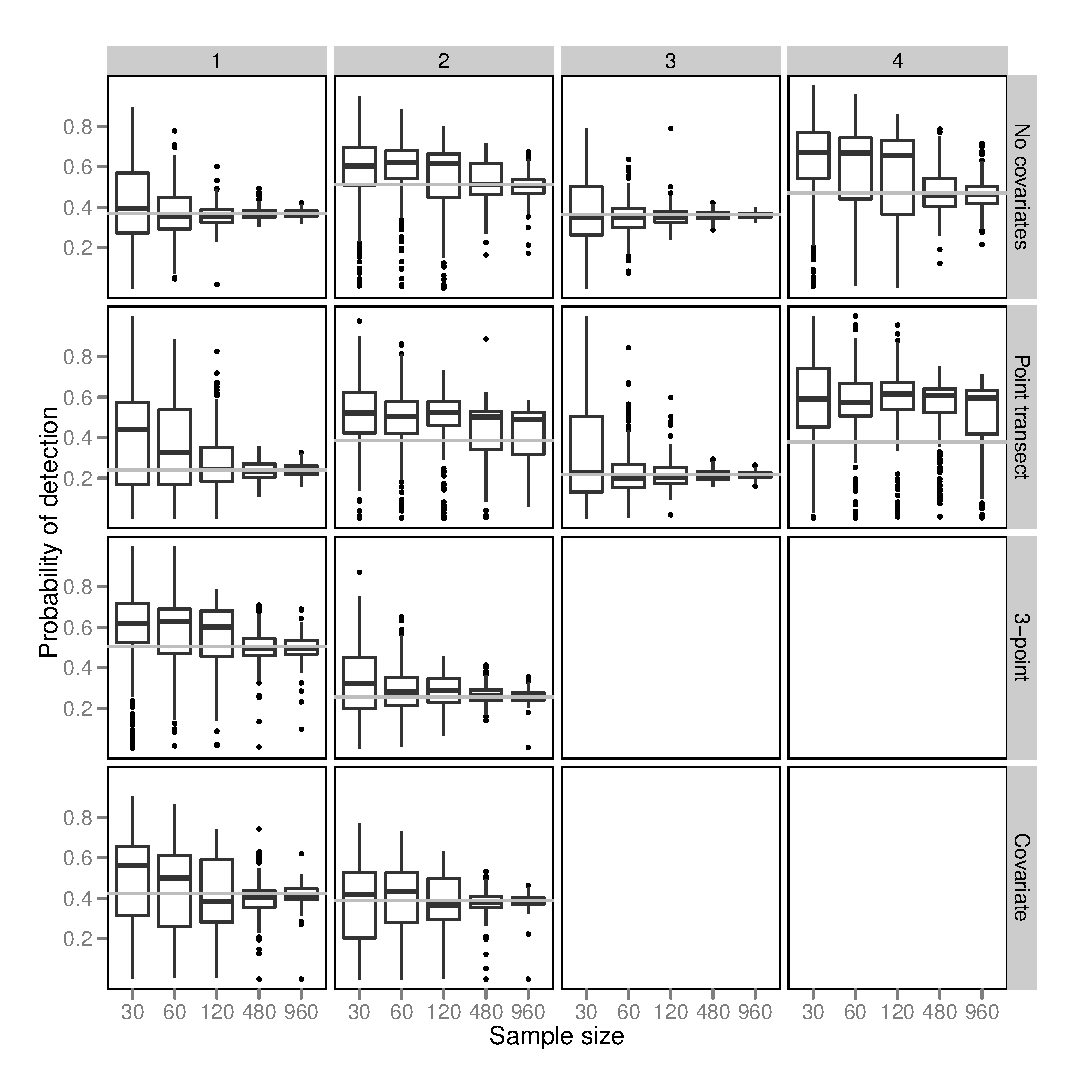
\includegraphics[width=\textwidth]{simulations/pa-plot.eps}
\caption{Simulation results: boxplots of the estimated detection probabilities for the best model (by AIC score). Layout is as in Figure \ref{sim-detfcts}. Grey lines indicate the true value of the average detection probability. Numbers underneath each boxplot give the proportion of AIC best models that were of the same form as the model that the data was simulated from (e.g. in covariate case 1 the proportion of AIC best models that were two point mixtures that included the covariate in the model).}
\label{sim-boxplots}
\end{figure}


\section{Real data}
\label{s:data}

Given the performance of the method in simulation, several data sets were analysed using the method. All of the analyses were performed in \texttt{mmds}, an \textsf{R} package written by the authors.

[[ Say something about mrds being used, Innes et al variances]]


[[\textbf{LEN}: is further detail needed for any of these?]]

\subsection{Williams and Thomas (2007) cetacean survey}

Williams and Thomas (2007) study several species of cetaceans off the coast of British Columbia. In particular look at the data for three species: harbour seal (in water), harbour porpoise and humpback whale (with truncation at 500, 500 and 2000m respectively). Results are summarised in Table \ref{williams-table} and detection functions for the best (in an AIC sense) models are shown in Figure \ref{williams-detfcts}.

\begin{table}
\caption{Comparison of the results for the Williams and Thomas (2007) data. W\&T indicates the results reported in Williams and Thomas (2007), other results are from mixture models where the number of mixture components was selected by AIC. $\cos(x)$ indicates a Cosine adjustment of order $x$.}
\centering
\begin{tabular}{c c c c c c}
\hline \hline
Species & Model & AIC & $\hat{P_a}$ & $\% CV \hat{P_a}$ & K-S $p$\\
\hline
Harbour seal & Hn+$\cos(2)$ (W\&T) & 2771.05 & 0.425 & 7.55 & 0.515\\
(in water) & Hn 2-pt  & 2769.86 & 0.335 & 14.8 & 0.945\\
Harbour porpoise & Hr (W\&T) & 690.66 & 0.212 & 32.0 & 0.99\\
 & Hn 2-pt & 692.09 & 0.254 & 17.5 & 0.99\\
Humpback & Hn+$\cos(2)$ (W\&T) & 1033.06 & 0.386 & 12.64 & 0.672 \\
 & Hn 2-pt & 1035.94 & 0.381 & 15.6 & 0.649 \\
\hline
\end{tabular}
\label{williams-table}
\end{table}

In each case a 2-point mixture was selected by AIC to be the best model. The mixture models for the harbour porpoise and the humpback both did not perform as well as the models selected in Williams and Thomas (2007). However, for the harbour porpoise the AIC is only different by 2, the detectability is very similar and the \%CV is lower, so it does not appear that much is lost by using the mixture model. In the case of the humpback, the fitted detection function is monotone, which was not the case in Williams and Thomas (2007); this added to the fact that there is again not a huge difference in results, leads us to believe that mixture models for the detection function can be useful. Finally, for the harbour seal data, the mixture model had a better AIC than the half-normal with cosine adjustments of order 2 which was selected in the paper. The goodness-of-fit was also significantly better than the result given in Williams and Thomas (2007).

\begin{figure}
\centering
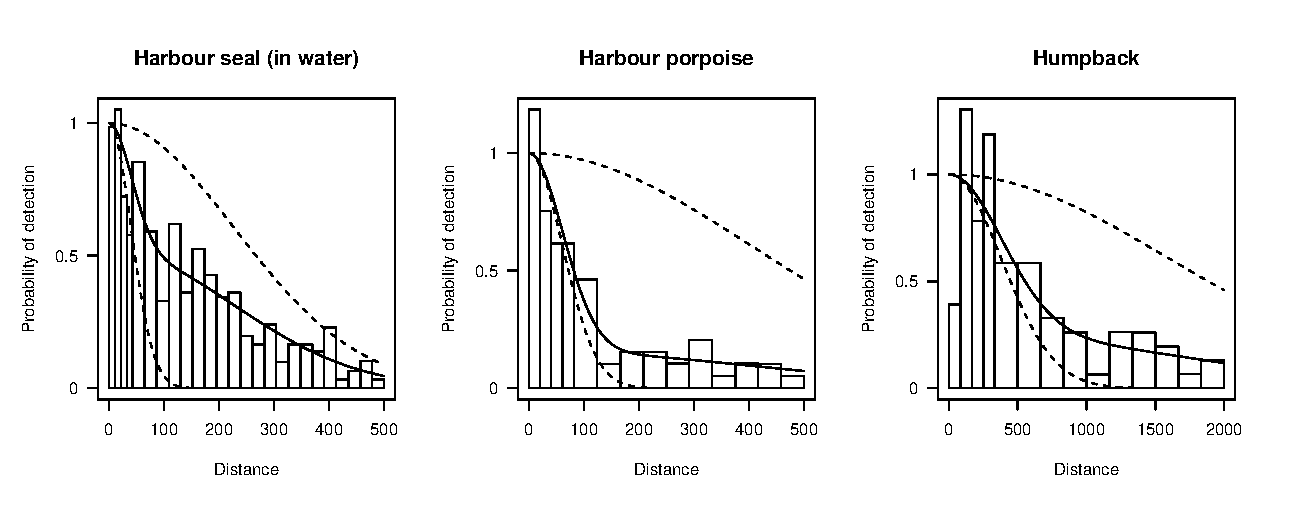
\includegraphics[width=\textwidth]{analyses/williamsplots.eps}
\caption{Plots of the detection functions fit to the Williams and Thomas (2007) data. In each case the best model by AIC was a 2-point mixture. Dashed lines show the mixture components.}
\label{williams-detfcts}
\end{figure}


\subsection{Wood ants in the Abernethy forest}

Borkin, Summers and Thomas (in press) analyse data on two species of wood ant (\textit{Formica aquilonia} and \textit{Formica lugubris}) in the Abernethy Forest in Strathspey Scotland over the period of August--September 2003. The number of nests sighted was 150 out to a distance of 72.04m from the track line, although 45\% of the nest sightings lay within 4m of the line. As part of their analysis several different truncation distances were used and larger truncation distances led to large variance in the encounter rate estimates and hence in overall abundance estimates (see Borkin et al., in press). This is due to the spike caused by the large number of detections close to the line.

As well as distances, three covariates were recorded: habitat type (\texttt{habitat}, a four level factor, the size (calculated as half-width multiplied by height) of each nest (\texttt{nest.size}, continuous variable) and whether \textit{Formica aquilonia} or \textit{Formica lugubris} were observed (\texttt{species}, a two level factor). In order to avoid numerical problems due to large values of the nest size, the variable was standardised.

As can be seen from Table \ref{big-results-table}, the best model by AIC was a 2-point mixture with nest size and habitat as covariates. This is not that surprising given the best CDS model (selected by AIC) in Distance was a hazard-rate with the same covariates. What is rather surprising is that the best mixture model had a better AIC than the hazard-rate, even though it has 1 more parameter. This is particularly encouraging since one might expect that mixtures would give good fits but would not achieve lower AIC scores due to the number of parameters required.

[[\textbf{LEN}: probably want to use the same binning here as in the paper?? Do you have it?]]

\begin{figure}
\centering
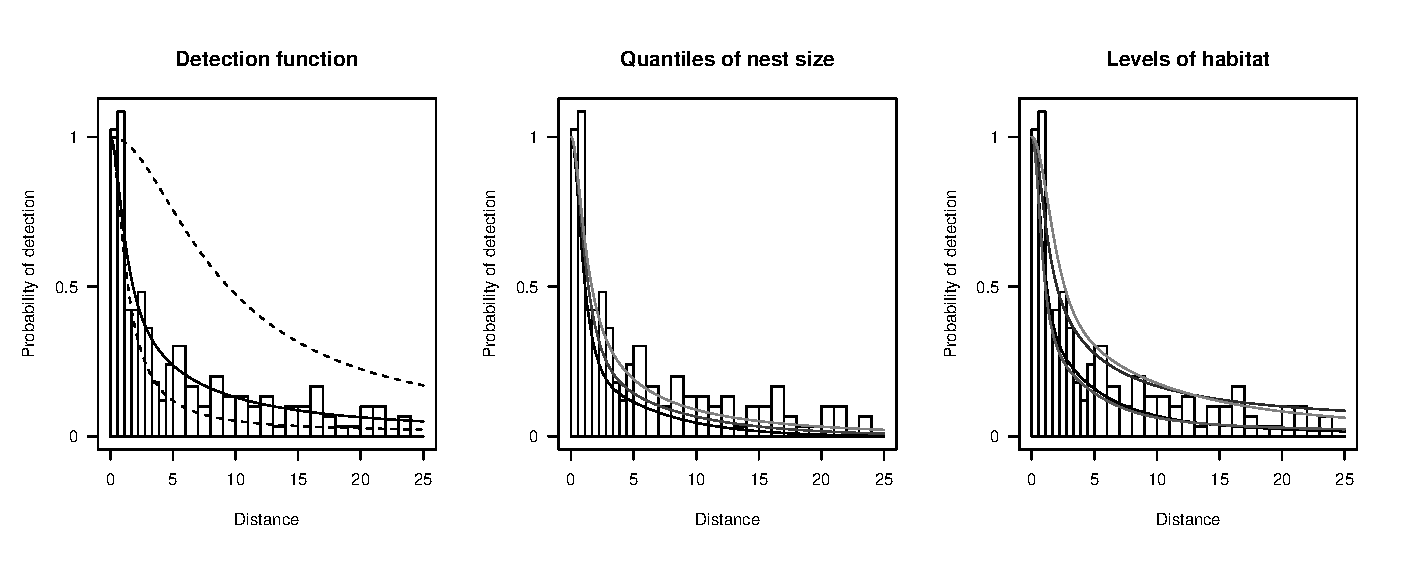
\includegraphics[width=\textwidth]{analyses/ants-nesthab.eps}
\caption{Plot of the detection functions for the AIC best model for the ants data set (2-point mixture with nest size and habitat as covariates). The first panel shows the average detection function (dashed lines are the two mixture components of the detection function, averaged over covariate values). The second and third panels show the quantiles (25\%, 50\% and 75\%) of nest size and the levels of habitat type respectively.}
\label{ants-nesthab}
\end{figure}


\subsection{Long-finned pilot whales}

Pike et al. (2003) analyse data on long-finned pilot whales (\textit{Globicephala melas}). There were 84 pods sighted as part of the NASS-2001 survey (of which the pilot whale was not a target). The Beaufort sea state was recorded as a covariate during the survey and enter the model as either a continuous variable (\texttt{BSS}), 6 level factor (\texttt{BSS}, as a factor), a 2 level factor (\texttt{BSS3}) or a 3 level factor (\texttt{BSS2}).

A model was fit with each of these covariates, as well as a model with no covariates. A summary of the results is given in Table \ref{big-results-table} and the detection function for the best model is shown in Figure \ref{danpike-detfct}.

\begin{figure}
\centering
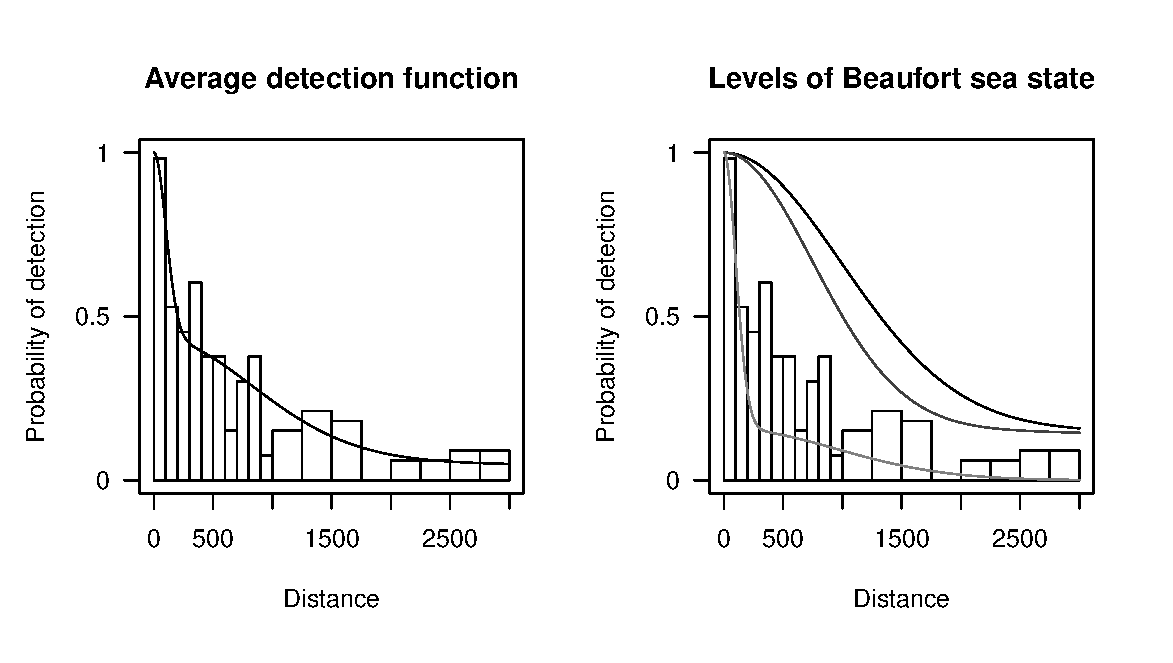
\includegraphics[width=0.75\textwidth]{analyses/danpike-bss2.eps}
\caption{The (AIC) best model for the long-finned pilot whale data -- a 2-point mixture model detection function with Beaufort sea state. Left: the average detection function, right: the marginal detection function with the levels of \texttt{BSS2}.}
\label{danpike-detfct}
\end{figure}

The best model by AIC score was a 2-point mixture with \texttt{BSS2} as a covariate. Figure \ref{danpike-detfct} shows the average detection function and the marginal detection function with the levels of \texttt{BSS2}.

\subsection{Amakihi}
Marques et al. (2007) analyse data on the Hawaii Amakihi (\textit{Hemignathus virens}). The data consist of 1485 observations on the bird ($n=1243$ after truncation at 82.5m), collected at 41 point transect from July 1992 to April 1995. Data was also collected on three covariates: the observer (\texttt{obs} , a three level factor), minutes after sunrise (\texttt{mas}, continuous) and hours after sunrise (\texttt{has}, a six level factor).

\begin{figure}
\centering
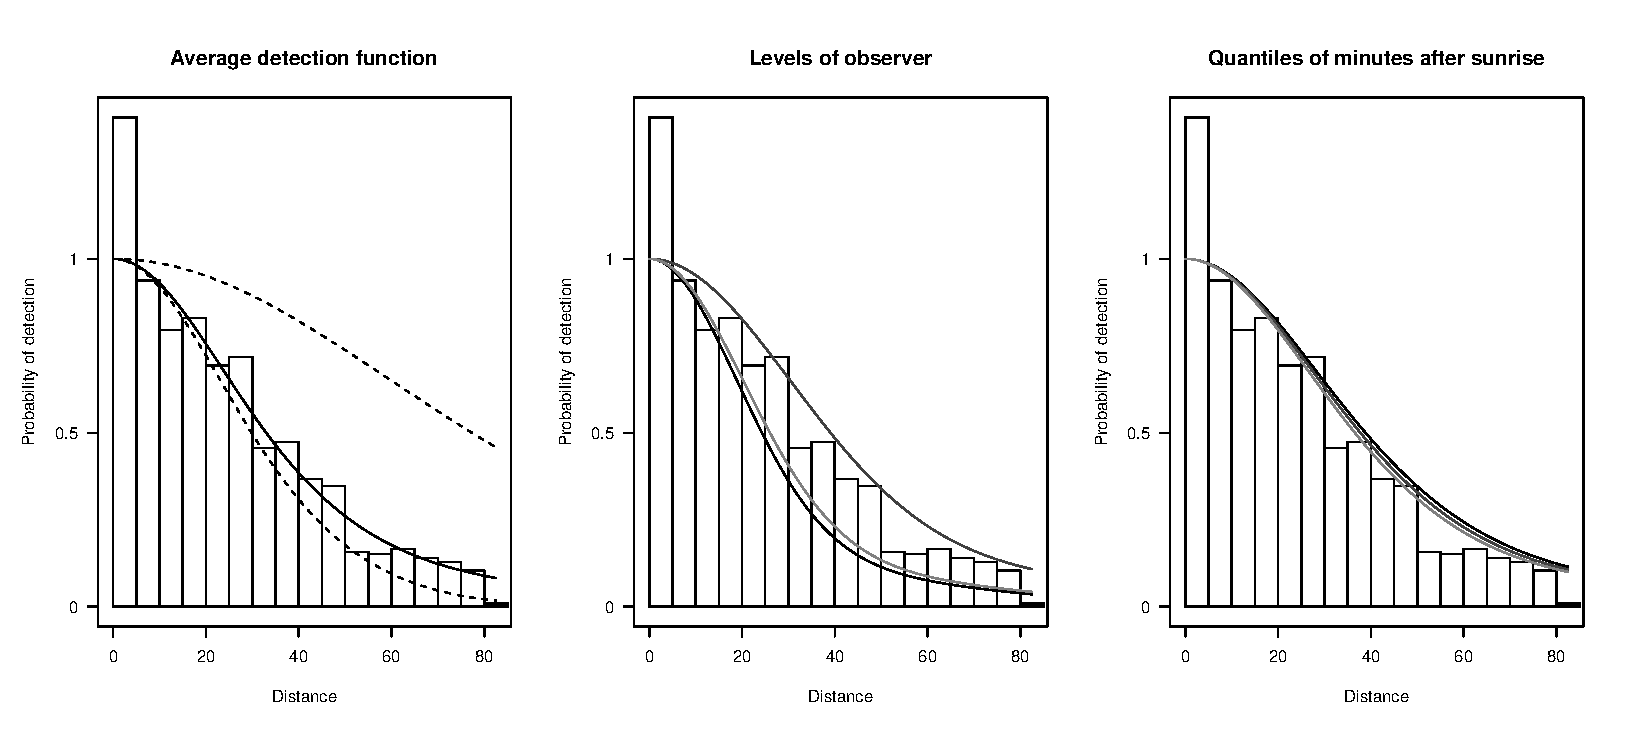
\includegraphics[width=\textwidth]{analyses/amakihi-om.eps}\\
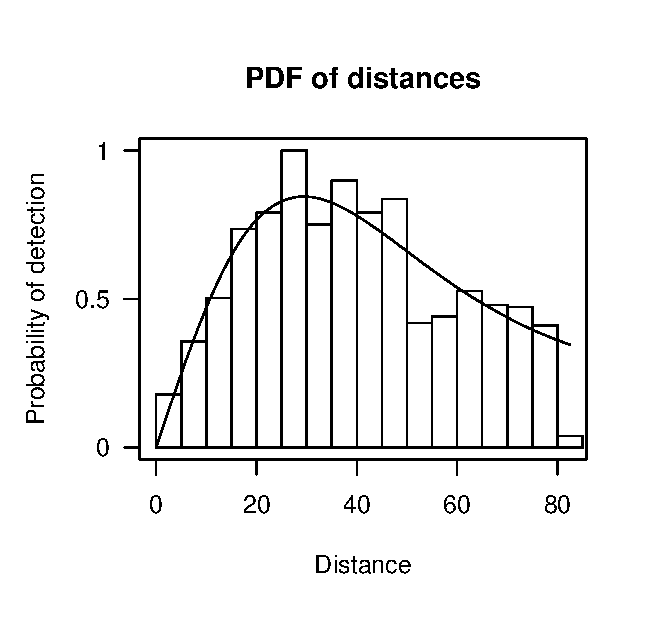
\includegraphics[width=0.4\textwidth]{analyses/amakihi-om-pdf.eps}
\caption{Plots of the (AIC) best model for the amakihi data. Top row: detection function averaged over covariates (dashed lines are each mixture component averaged over covariates), marginal detection function showing the levels of observer (averaged over the values of minutes after sunrise) and marginal detection function for the quantiles minutes after sunrise (averaged over the levels of observer). Bottom row: pdf of distances averaged over the covariate values.}
\label{amakihi}
\end{figure}

Best mixture model according to AIC was a two point mixture with observer and minutes after sunrise as covariates (shown in Figure \ref{amakihi}), closely followed by the model with only observer as a covariate (see Table \ref{big-results-table}). In this case a hazard-rate with observer and minutes after sunrise as covariates beat the mixtures in AIC terms. This is not too surprising given that the mixtures use one more parameter than a hazard-rate in this situation. It is encouraging that there is such a small difference in AIC, and that covariate mixture models were selected despite the large number of parameters that such models entail.


\begin{table}
\caption{Results for the three data sets with covariates. Bold indicates lowest AIC for each set. In each set the final model is the lowest AIC model reported in the original analysis (in Distance). Kolmogorov-Smirnov test $p$-values (KS $p$) are also given as in Section 11.11 of Buckland \textit{et al.} (2004). Results are from ($i$) the wood ant data from Borkin \textit{et al.} with truncation at 25m; ($ii$) the long-finned pilot whales Pike et al. (2003) with truncation at 3000m, (cont.) denotes that the covariate was included in the model as continuous, otherwise covariates entered the model as factors; ($iii$) the amakihi data from Marques et al. (2007) with truncation at 82.5m.}
\centering
\begin{tabular}{c l c c c c}
\hline \hline
Model & Covariates & AIC & $\hat{P_a}$ & $\% CV \hat{P_a}$ & K-S $p$\\
\hline
 & ($i$) \textit{Ants} & & & & \\
Hn 2-pt & None & 754.61 & 0.183 & 16.2 & 0.96 \\
Hn 2-pt & \texttt{habitat} & 751.27 & 0.150 & 20.2 & 0.97 \\ 
Hn 2-pt & \texttt{species} & 756.59 & 0.184 & 16.35 & 0.94 \\  
Hn 2-pt & \texttt{nest.size} & 741.64 & 0.214 & 15.71 & 0.76 \\   
Hn 2-pt & \texttt{habitat} + \texttt{species} & 749.05 & 0.152 & 19.85 & 0.94\\ 
Hn 2-pt & \texttt{habitat} + \texttt{nest.size} & \textbf{737.27} & 0.179 & 22.47 & 0.72\\
Hn 2-pt & \texttt{nest.size} + \texttt{species} & 741.92 & 0.210 & 18.09 & 0.77\\
Hn 2-pt & \texttt{nest.size} + \texttt{species} + \texttt{habitat} & 739.77 & 0.178 & 18.9 & 0.68 \\
% Hr & \texttt{nest.size} + \texttt{habitat} & 745.2 & 0.194 & 10.6 & 0.95\\  % Distance result 
Hr & \texttt{nest.size} + \texttt{habitat} & 743.56 & 0.195  & 21.72 & 0.89\\ % mrds result
 & ($ii$) \textit{Long-finned pilot whales} & & & & \\
Hn 2-pt & None & 1298.42 & 0.295 & 23.6 & 0.95 \\
Hn 2-pt & \texttt{BSS} & 1286.6 & 0.209 & 22.06 & 0.82 \\
Hn 2-pt & \texttt{BSS2} & \textbf{1284.99} & 0.211 &  22.05 & 0.95\\
Hn 2-pt & \texttt{BSS3} & 1296.27 & 0.27 & 24.8 & 0.99 \\
Hn 2-pt & \texttt{BSS} (cont.) &  1286.26 & 0.152 & 44.1 & 0.84\\
% Hn 1-pt + $\cos(2)$& \texttt{BSS} (cont.) & 1296 & 0.37 & 9.56 & 0.319 \\ % Distance result 
Hn 1-pt + $\cos(2)$& \texttt{BSS} (cont.) & 1286.5 & 0.452 & 8.69 & \\ % mrds
 & ($iii$) \textit{Amakihi} & & & & \\
Hn 2-pt & None & 10805.48 & 0.28 & 5.14 & 0.12 \\
Hn 2-pt & \texttt{obs} & 10778.69 & 0.28 & 5.8 & 0.04\\
Hn 2-pt & \texttt{has} & 10807.19 &  0.28 & 6.48 & 0.33\\
Hn 2-pt & \texttt{mas} & 10805.11 &  0.28 & 5.96 & 0.31\\
Hn 2-pt & \texttt{obs} + \texttt{has} & 10782.53 & 0.28 & 6.88 & 0.23\\
Hn 2-pt & \texttt{obs} + \texttt{mas} & 10778.07 & 0.28 & 5.93 & 0.14\\
Hn 2-pt & \texttt{has} + \texttt{mas} & 10809.17 & 0.28 & 6.53 & 0.43 \\
Hn 2-pt & \texttt{obs} + \texttt{has} + \texttt{mas} & 10784.5 & 0.28 & 7.62 & 0.35\\
% Hr & \texttt{obs} + \texttt{mas} & \textbf{10777.72} & 0.3 & 2.65 & 0.036 \\ % Distance result 
Hr & \texttt{obs} + \texttt{mas} & \textbf{10777.38} &  0.319 & 5.11 & 0.076\\ % mrds
\hline
\hline
\end{tabular}
\label{big-results-table}
\end{table}

%Amakihi
%6.2 
%5.85 
%6.95 
%6.52 
%6.21 
%6.1 
%6.97 
%6.33 




\section{Discussion}
\label{s:discuss}

[[\textbf{LEN}: I've put some stuff here but it's a bit rough at the moment. ]]

The article has investigated and demonstrated the utility of detection functions constructed from mixtures of half-normals in both line and point transect distance sampling. We also show that covariates can be included in such models easily. These mixture detection functions can be simply ``dropped in'' to the existing theory.

We have shown that the method performs well on both simulated and real data. In many cases the proposed model outperforms the existing CDS models, which is surprising given that the mixture models in question often had more parameters than the CDS models. It should be noted however, that in simulation at small sample sizes models will not fit data generated from them particularly well. We avoid this problem by using AIC forward selection for the number of mixtures, ensuring model parsimony.

In simulation we observed that using a 3-point mixture was not a good surrogate for missing covariate structure in the model. We also saw that 2-point mixtures were generally chosen by AIC as good models and that the construction of a true 3-point mixture is quite tricky. In the examples in section \ref{s:data}, 2-point mixtures consistently provided the best fit, even in the case of the amakihi which was a very large data set ($n=1243$). Only examination of further data will show whether 3-point and higher mixtures can be supported in real data, however we note that in CDS when the key function with adjustment series formulation is used, detection functions with $5$ or more parameters are rarely selected by AIC and a 3-point mixture with no covariates requires $5$ parameters.

All the models discussed in this article are available as an \textsf{R} package, \texttt{mmds} which is available from \url{http://www.github.com/dill/mmds/}.

[[\textbf{LEN}: Will be in next version of Distance?!]]

[[\textbf{LEN}: Not sure about this yet, need to think about it...]]

Further work will include extending these models further to include continuous mixtures. In that case the detection function can be modelled as:
\begin{equation*}
g(x) = \int_\mathbf{R} \varphi(\kappa) g_\kappa(x,\mathbf{Z}; \theta, \kappa) \text{d}\kappa
\end{equation*}
where $\varphi(\kappa)$ is some function which controls the mixing of $g_\kappa$. Such an approach may present significant computation issues, however the benefits for model fitting may be considerable. Provided that an appropriate function can be chosen for $\varphi$, more flexible models could be used whilst keeping the number of parameters low. In addition, a combination of both finite and continuous mixtures could be used, echoing the work of Morgan and Ridout (2008) in capture-recapture.


%  The \backmatter command formats the subsequent headings so that they
%  are in the journal style.  Please keep this command in your document
%  in this position, right after the final section of the main part of 
%  the paper and right before the Acknowledgements, Supplementary Materials,
%  and References sections. 

\backmatter

%  This section is optional.  Here is where you will want to cite
%  grants, people who helped with the paper, etc.  But keep it short!

\section*{Acknowledgements}

David would like to acknowledge the (financial) support of EPSRC and Simon N. Wood for useful discussions.

Both authors would like to thank David Borchers, who suggested the parametrisation for the mixture proportions as well as\ldots

Rob Williams, Dan Pike , the amakihi people and the ant people for the data. [[\textbf{LEN}: can you put in the right people to thank here?]]


%  Here, we create the bibliographic entries manually, following the
%  journal style.  If you use this method or use natbib, PLEASE PAY
%  CAREFUL ATTENTION TO THE BIBLIOGRAPHIC STYLE IN A RECENT ISSUE OF
%  THE JOURNAL AND FOLLOW IT!  Failure to follow stylistic conventions
%  just lengthens the time spend copyediting your paper and hence its
%  position in the publication queue should it be accepted.

%  We greatly prefer that you incorporate the references for your
%  article into the body of the article as we have done here 
%  (you can use natbib or not as you choose) than use BiBTeX,
%  so that your article is self-contained in one file.
%  If you do use BiBTeX, please use the .bst file that comes with 
%  the distribution.

\begin{thebibliography}{}

\bibitem{ } Beavers, S. C., and Ramsey, F. L. (1998). Detectability analysis in transect surveys. \textit{Journal of Wildlife Management} \textbf{62}(3), pp. 948--957.

\bibitem{ } Becker, E. F. and Quang, P. X. (2009). A gamma-shaped detection function for line-transect surveys with mark-recapture and covariate data. \textit{Journal of Agricultural, Biological, and Environmental Statistics} \textbf{14}(2), 207--223.

\bibitem{ } Borkin, K., Summers, R. and Thomas, L. (\textit{in press}). Surveying abundance and stand type associations of wood ant Formica spp.(Hymenoptera: Formicidae) nest mounds over an extensive area: trialing a novel method. European Journal of Entomology.

\bibitem{ } Buckland, S.T. (1992). Fitting density functions using polynomials. \textit{Applied Statistics} \textbf{41}, 63--76. 

\bibitem{ }  Buckland, S. T., Anderson, D. R., Burnham, K. P., Laake, J. L., Borchers, D. L., and Thomas, L.  (2001). \textit{Distance Sampling}. Oxford University Press. Oxford, UK.

\bibitem{ }  Buckland, S. T., Anderson, D. R., Burnham, K. P., Laake, J. L., Borchers, D. L., and Thomas, L.  (2004). \textit{Advanced Distance Sampling}. Oxford University Press. Oxford, UK.

\bibitem{ } Dempster, A.P., Laird,  N. M. and Rubin, D. B. (1977). Maximum Likelihood from Incomplete Data via the EM Algorithm. \textit{Journal of the Royal Statistical Society: Series B (Methodological)} \textbf{39}(1), 1--38.

\bibitem{ } Dorazio, R. M. and Royle, J. A. (2003) Mixture Models for Estimating the Size of a Closed Population When Capture Rates Vary among Individuals. \textit{Biometrics} \textbf{59}(2), 351--364 

\bibitem{ }  Gelman, A., Carlin, J. B., Stern, H. S., and Rubin, D. B. (2004). \textit{Bayesian Data Analysis}. CRC Press. Boca Ranton, Florida, US.

\bibitem{ } Mack, Y. P. and Quang, P. (1998). Kernel methods in line and point transect sampling. \textit{Biometrics} \textbf{54}(2), 606--619. 

\bibitem{ } Marin, J. M., Mengersen, K. and Robert, C. P. (2005). Bayesian modelling and inference on mixtures of distributions. \textit{Handbook of Statistics 25} D. Dey and C.R. Rao (eds). Elsevier-Sciences.

\bibitem{ } Marques, T. A., Thomas, L., Fancy, S. G., Buckland, S. T. (2007). Improving estimates of bird density using multiple-covariate distance sampling. \textit{The Auk} \textbf{124}(9), 1229--1243.

\bibitem{ } Morgan, B. J. T. and Ridout, M. (2008). A new mixture model for capture heterogeneity. \textit{Journal of the Royal Statistical Society: Series C} \textbf{57}(4), 433--446. 

\bibitem{ } Pike, D. G., Gunnlaugsson, T., V\'{i}kingsson, G .A., Desportes, G. and Mikkelson, B.  (2003) An estimate of the abundance of long-finned pilot whales (\textit{globicephala melas}) from the NASS-2001 shipboard survey. Paper SC/11/AE/10 presented to the North Atlantic Marine Mammal Commission (NAMMCO) Scientific Committee Working Group on Abundance Estimates.

\bibitem{ } Pledger, S. (2000). Unified maximum likelihood estimates for closed capture-recapture models using mixtures. \textit{Biometrics} \textbf{56}(2), 434--442. 

\bibitem{ } Pledger, S. (2005). The performance of mixture models in heterogeneous closed population capture-recapture. \textit{Biometrics} \textbf{61}(3), 868--873.

\bibitem{ } Thomas, L., Buckland, S. T., Rexstad, E. A., Laake, J. L., Strindberg, S., Hedley, S. L., Bishop, J. R. B., Marques, T. A. and Burnham, K. P. (2010). Distance software: design and analysis of distance sampling surveys for estimating population size. \textit{Journal of Applied Ecology} \textit{47}, 5--14.

\bibitem{ } Thompson, S. K. (2002). \textit{Sampling}. Wiley, New York, US.

\bibitem{ } Williams, R. and Thomas, L. (2007). Distribution and abundance of marine mammals in the coastal waters of British Columbia, Canada. \textit{Journal of Cetacean Research and Management} \textbf{9}(1), pp. 15--38.

\end{thebibliography}


\section*{Appendix A - Optimization}
\label{s:optimization}

As noted in the literature (e.g. Gelman et al, 2004, Marin, Mengersen, Robert, 2005]], mixture model likelihoods can be notoriously multimodal. This can cause serious problems when finding MLEs of the parameters. Here simulated annealing was used to explore the parameter space (for 500 iterations) then after that BFGS was used to find the maxima (the implementations in the \textsf{R} function \texttt{optim()} were used). These two steps were run 5 times. This two step approach appears to be satisfactory in most cases. The EM algorithm (Dempster, Laird and Rubin, 1977) was also used although there was no significant performance increase (in terms of computational time or parameter precision) over using BFGS with SANN. To aid the optimization, analytic derivatives were also found; these can be found in appendix B.

\subsection{Starting values}
Beavers and Ramsay (1998) give a method for estimating starting values for the scale parameter of a half-Normal detection function. In the non-covariate case, the estimate is given as the intercept parameter from intercept only regression on $\log(x+\frac{w}{1000})$ (where $w$ denotes the truncation distance, as above). For covariate models, the equation used for the $\sigma$ is used in the regression and the estimated parameters from the linear regression are used as the starting values for the $\beta$s.

A similar approach can be use in the mixture case by dividing the sorted distances into $J$ equal parts. For each of these parts a Beavers and Ramsay-type estimate is used for the $\beta$s. The $\phi_j$ had starting values of $1/J$ since there is no reason \textit{a priori} to believe anything else.

\subsection{Parametrisation of the mixture proportions}

When using 2-point mixtures, the constraint that the mixture proportions must sum to unity is enforced by definition (since $\phi_2=1-\phi_1$). However, in $J$-point mixtures when $J>2$ ensuring that the proportions sum to 1 is not guaranteed. The obvious way to get around this would be to penalise the likelihood, should the optimisation procedure propose values for the $\phi_j$s that are not in accordance with this condition. This is, of course, inefficient and ugly. Instead, a parametrisation is used for the mixture proportions which yields $\phi_j$s that comply.

Rather than estimating the $\phi_j$s, estimate $\alpha_p$s, where the relationship between the two is:
\begin{equation*}
\phi_j = F(\sum_{p=1}^j e^{\alpha_p}) - F(\sum_{p=1}^{j-1} e^{\alpha_p}) \qquad \text{for } 1\leq j \leq J-1
\end{equation*}
and
\begin{equation*}
\phi_J = 1-\sum_{j=1}^{J-1} \phi_j
\end{equation*}
where $F$ is any continuous CDF on $(0,\infty]$. Exponentiation ensures that $e^{\alpha_p}\geq0$, so $\alpha_p$ may lie anywhere on the real line, allowing unconstrained optimisation. Summing these orders the $\phi_j$s, since only offsets are estimated. Finally, using the cumulative density function ensures that the $\phi_j$s sum to $1$. In practise the $\text{Gamma}(3,2)$ CDF is (somewhat arbitrarily) used. Figure [[TKTKTK figure -- do we need this?]] illustrates the relationship.

To transform from the $\phi_j$s back to the $\alpha_p$s we simply re-arrange the above expression.
\begin{equation*}
\alpha_p = \log_e \Big(F^{-1}\Big(\phi_j + F(\sum_{p=1}^{j-1} e^{\alpha_p})\Big) - \sum_{p=1}^{j-1} e^{\alpha_p}\Big).
\end{equation*}
Note that we only need as many $\alpha_p$s as we had $\phi_j$s, so we do not require any additional parameters.

\section*{Appendix B - Derivatives}

\begin{equation}
l(\bm{\theta}, \bm{\phi}; \mathbf{r},\mathbf{Z}) = n \log 2 \pi + \sum_{i=1}^n \Big( \log r_i + \log \sum_{j=1}^J \phi_j g_j(r_i,\mathbf{Z}; \bm{\theta}_j) - \log \sum_{j=1}^J \phi_j \nu_{ij}\Big)
\label{pt-lik}
\end{equation}
\begin{equation}
l(\bm{\theta}, \bm{\phi}; \mathbf{x},\mathbf{Z}) = \sum_{i=1}^n \Big( \log \sum_{j=1}^J \phi_j g_j(x_i,\mathbf{Z}; \bm{\theta}_j) - \log \sum_{j=1}^J \phi_j \mu_{ij}\Big)
\label{lt-lik}
\end{equation}


\subsection*{Line transects}

Starting from the likelihood given in (\ref{lt-lik}), we derive the derivatives with respect to the optimisation parameters.

\subsection*{With respect to $\beta_{0j*}$}
For the intercept terms (also considering in the non-covariate case, these are just the parameters), the parameters have no effect outside of their mixture (ie. $\beta_{0j*}$ only has an influence on mixture component $j*$), so we can write:
\begin{equation*}
\frac{\partial l(\bm{\theta},\bm{\phi}; \mathbf{x},\mathbf{Z})}{\partial \beta_{0j*}} = \sum_{i=1}^n \frac{1}{g(x_i,\mathbf{Z}; \bm{\theta},\bm{\phi})} \phi_{j*} \frac{\partial}{\partial \beta_{0j*}} g_{j*}(x_i,\mathbf{Z}; \bm{\theta}_{j*})  - \frac{\phi_{j*}}{\mu_i}  \frac{\partial}{\partial \beta_{0j*}} \mu_{ij*}.
\end{equation*}
Now, to first fine $\frac{\partial}{\partial \beta_{0j*}} g_{j*}(x_i,\mathbf{Z}; \bm{\theta}_{j*})$:
\begin{equation*}
\frac{\partial g_{j*}(x_i,\mathbf{Z}; \bm{\theta}_{j*})}{\partial \beta_{0j*}} = \frac{\partial}{\partial \beta_{0j*}} \exp\Big( -\frac{x_i^2}{2\sigma_{j*}^2} \Big)
\end{equation*}
applying the chain rule and remembering that $\sigma_{j*}$ is a (trivial) function of the $\beta_{0j}$s:
\begin{equation*}
\frac{\partial g_{j*}(x_i,\mathbf{Z}; \bm{\theta}_{j*})}{\partial \beta_{0j*}} = \Big( \frac{x_i}{\sigma_{j*}}\Big)^2 \exp \Big(-\frac{x_i^2}{2 \sigma_{j*}^2}\Big)
\end{equation*}

Expressing $\mu_{ij*}$ in terms of the error function:
\begin{align}
\frac{\partial \mu_{ij*}}{\partial \beta_{0j*}} &= \frac{\partial}{\partial \beta_{0j*}} \Big( \sqrt{\frac{\pi}{2}} \sigma_{j*} \text{Erf}\Big(\frac{w}{\sqrt{2\sigma_{j*}^2}}\Big) \Big) \notag \\
&= \text{Erf}\Big(\frac{w}{\sqrt{2\sigma_{j*}^2}}\Big) \frac{\partial}{\partial \beta_{0j*}} \Big( \sqrt{\frac{\pi}{2}} \sigma_{j*} \Big) + \sqrt{\frac{\pi}{2}} \sigma_{j*} \frac{\partial}{\partial \beta_{0j*}} \Big(\text{Erf}\Big(\frac{w}{\sqrt{2\sigma_{j*}^2}}\Big) \Big)\label{app-mu-erf}
\end{align}
To find $\frac{\partial}{\partial \beta_{0j*}} \text{Erf}\Big(\frac{w}{\sqrt{2\sigma_{j*}^2}}\Big)$, note that we can write and then apply the chain rule:
\begin{align*}
\frac{\partial}{\partial \beta_{0j*}} \text{Erf}\Big(\frac{w}{\sqrt{2\sigma_{j*}^2}}\Big) &= \frac{\partial}{\partial \beta_{0j*}} S(u(\sigma_{j*}))\\
&= \frac{\partial S(u)}{\partial u} \frac{\partial u(\sigma_{j*})}{\partial \sigma_{j*} } \frac{\partial \sigma_{j*}}{\partial \beta_{0j*}}
\end{align*}
where 
\begin{align*}
S(u) = \int_0^{u} \exp(-t^2) \text{d}t \quad \text{and} \quad u(\sigma_{j*})=\frac{w}{\sqrt{2\sigma_{j*}^2}}.
\end{align*}
Their derivatives being
\begin{align*}
\frac{\partial S(u)}{\partial u} = \frac{2}{\sqrt{\pi}} \exp(-u^2) \text{,} \quad \frac{\partial u(\sigma_{j*})}{\partial \sigma_{j*}} = -\frac{w}{\sqrt{2}}\sigma_{j*}^{-2}.
\end{align*}
Given these terms, it's just a case of multiplying them:
\begin{align*}
\frac{\partial S(u)}{\partial u} \frac{\partial u(\sigma_{j*})}{\partial \sigma_{j*} } \frac{\partial \sigma_{j*}}{\partial \beta_{0j*}} = - \sqrt{\frac{2}{\pi}} \frac{w}{\sigma_{j*}} \exp\Big( -\frac{w^2}{2\sigma_{j*}^2} \Big)
\end{align*}
Substituting into (\ref{app-mu-erf}):
\begin{equation*}
\frac{\partial \mu_{ij*}}{\partial \beta_{0j*}} =  \mu_{ij*} - w \exp\Big( -\frac{w^2}{2\sigma_{j*}^2} \Big)
\end{equation*}
Finally, the derivative is:
\begin{equation*}
\frac{\partial l(\bm{\theta}, \bm{\phi}; \mathbf{x},\mathbf{Z})}{\partial \beta_{0j*}} = \sum_{i=1}^n \Big( \frac{x_i}{\sigma_{j*}}\Big)^2 \phi_{j*} \frac{g_{j*}(x_i,\mathbf{Z}; \bm{\theta}_{j*})}{g(x_i,\mathbf{Z}; \bm{\theta},\bm{\phi})}  - \frac{\phi_{j*}}{\mu_i} (\mu_{ij*} - w g_{j*}(w,\mathbf{Z}; \bm{\theta}_{j*})).
\end{equation*}



\subsection*{With respect to $\beta_{k*}$}

Derivatives with respect to the common covariate parameters are found in a similar way to above. The expressions are slightly more complicated since the $\beta_k$s effect all of the mixture components.
\begin{equation*}
\frac{\partial l(\bm{\theta},\bm{\phi}; \mathbf{x},\mathbf{Z})}{\partial \beta_{k*}} = \sum_{i=1}^n \Big( \frac{1}{g(x_i,\mathbf{Z}; \bm{\theta},\bm{\phi})} \sum_{j=1}^J \phi_j \frac{\partial}{\partial \beta_{k*}} g_j(x_i,\mathbf{Z}; \bm{\theta}_j) - \frac{1}{\mu_i} \sum_{j=1}^J \phi_j \frac{\partial}{\partial \beta_{k*}}\mu_{ij}\Big)
\end{equation*}
Every $\sigma_{j}$ is a function of the $\beta_{k}$s, so:
\begin{align*}
\frac{\partial \sigma_{j}}{\partial \beta_{k*}} &= \frac{\partial}{\partial \beta_{0j*}} \exp \Big( \beta_{0j} + \sum_{k=1}^K z_{ik} \beta_{k}\Big),\\
&= z_{ik*} \exp \Big( \beta_{0j} + \sum_{k=1}^K z_{ik} \beta_{k}\Big),\\
&= z_{ik*}\sigma_{j}.
\end{align*}
Hence:
\begin{equation*}
 \frac{\partial}{\partial \beta_{k*}} \exp\Big( -\frac{x_i^2}{2\sigma_{j}^2} \Big) = z_{k*} \Big( \frac{x_i}{\sigma_{j}}\Big)^2 \exp \Big(-\frac{x_i^2}{2 \sigma_{j}^2}\Big) = z_{k*} \Big( \frac{x_i}{\sigma_{j}}\Big)^2 g_j(x_i,\mathbf{Z}; \bm{\theta}_j).
 \label{detfct-deriv-k}
\end{equation*}
And so for the $\mu_{ij}$s:
\begin{equation*}
\frac{\partial \mu_{ij}}{\partial \beta_{k*}} = z_{ik*} \Big( \mu_{ij} - w \exp\Big( -\frac{w^2}{2\sigma_{j}^2} \Big) \Big)
\end{equation*}
The derivative is then:
\begin{equation*}
\frac{\partial l(\bm{\theta},\bm{\phi}; \mathbf{x},\mathbf{Z})}{\partial \beta_{k*}} = \sum_{i=1}^n \Big( \frac{1}{g(x_i,\mathbf{Z}; \bm{\theta},\bm{\phi})} \sum_{j=1}^J \phi_j  z_{k*} \Big( \frac{x_i}{\sigma_{j}}\Big)^2 g_j(x_i,\mathbf{Z}; \bm{\theta}_j) - \frac{1}{\mu_i} \sum_{j=1}^J \phi_j z_{ik*} ( \mu_{ij} - w g_j(x_i,\mathbf{Z}; \bm{\theta}_j) )\Big)
\end{equation*}

\subsubsection*{With respect to $\alpha_{j*}$}

First note that we can write the likelihood (\ref{lt-lik}) as:
\begin{align*}
l(\bm{\theta},\bm{\phi}; \mathbf{x},\mathbf{Z}) = \sum_{i=1}^n\Big( &\log \Big( \sum_{j=1}^{J-1} \phi_j g_j(x_i,\mathbf{Z}; \bm{\theta}_j) + (1-\sum_{j=1}^{J-1} \phi_j) g_J(x_i,\mathbf{Z}; \bm{\theta}_J)\Big) \\
&-  \log \Big(\sum_{j=1}^{J-1} \phi_j \mu_{ij} + (1-\sum_{j=1}^{J-1} \phi_j) \mu_{ij} \Big) \Big)
\end{align*}
The derivatives with respect to the $\alpha_{j*}$ of this expression are then:
\begin{align}
\frac{\partial l(\bm{\theta},\bm{\phi}; \mathbf{x},\mathbf{Z})}{\partial \alpha_{j*}} = &\Big( \sum_{i=1}^n \frac{1}{g(x_i,\mathbf{Z}; \bm{\theta},\bm{\phi})} \Big( \sum_{j=1}^{J-1} g_j(x_i,\mathbf{Z}; \bm{\theta}_j) \frac{\partial \phi_j}{\partial \alpha_{j*}}  -g_J(x_i,\mathbf{Z}; \bm{\theta}_J) \sum_{j=1}^{J-1}  \frac{\partial \phi_j}{\partial \alpha_{j*}}\Big) \notag \\
&- \frac{1}{\mu_i} \Big(\sum_{j=1}^{J-1} \mu_{ij} \frac{\partial \phi_j}{\partial \alpha_{j*}} - \mu_{iJ} \sum_{j=1}^{J-1}   \frac{\partial \phi_j}{\partial \alpha_{j*}} \Big)\Big) \label{app-lik-alphad}
\end{align}
Finding the derivatives is then simply a matter of finding the derivatives of $\phi_{j}$ with respect to $\alpha_{j*}$ and substituting them back into (\ref{app-lik-alphad}).
\begin{equation*}
\frac{\partial \phi_j}{\partial \alpha_{j*}} = \frac{\partial}{\partial \alpha_{j*}}F(\sum_{p=1}^j e^{\alpha_p}) - \frac{\partial}{\partial \alpha_{j*}} F(\sum_{p=1}^{j-1} e^{\alpha_p}).
\end{equation*}
Looking at each of the terms:
\begin{equation*}
\frac{\partial}{\partial \alpha_{j*}} F(\sum_{p=1}^j e^{\alpha_p})=A_{j}=\begin{cases}
e^{\alpha_{j*}}f(\sum_{p=1}^j e^{\alpha_p})& \text{for $j\geq j*$},\\
0 & \text{for $j<j*$}.
\end{cases}
\end{equation*}
and
\begin{equation*}
\frac{\partial}{\partial \alpha_{j*}} F(\sum_{p=1}^{j-1} e^{\alpha_p})=A_{(j-1)}=\begin{cases}
e^{\alpha_{j*}}f(\sum_{p=1}^{j-1} e^{\alpha_p})& \text{for $j-1\geq j*$},\\
0 & \text{for $j-1<j*$}.
\end{cases}
\end{equation*}
So
\begin{equation*}
\frac{\partial \phi_j}{\partial \alpha_{j*}} = A_j - A_{j-1}.
\end{equation*}
Substituting these back into (\ref{app-lik-alphad}) and re-arranging gives:
\begin{align*}
\frac{\partial l(\bm{\theta},\bm{\phi}; \mathbf{x},\mathbf{Z})}{\partial \alpha_{j*}} = \sum_{i=1}^n & \Big( \frac{1}{g(x_i,\mathbf{Z}; \bm{\theta},\bm{\phi})} \sum_{j=1}^{J-1} (A_j - A_{j-1}) (g_j(x,\mathbf{Z}; \bm{\theta}_j) - g_J(x,\mathbf{Z}; \bm{\theta}_J))\\
&- \frac{1}{\mu_i} \sum_{j=1}^{J-1}(A_j - A_{j-1})(\mu_{ij} - \mu_{iJ}) \Big)
\end{align*}

\subsection*{Point transects}

\subsubsection*{With respect to $\beta_{0j}$}

Starting with the likelihood in (\ref{pt-lik}), one can see that we obtain:
\begin{align*}
\frac{\partial l(\bm{\theta}, \bm{\phi}; \mathbf{r},\mathbf{Z})}{\partial \beta_{0j*}}  &= \sum_{i=1}^n \Big( \frac{\partial}{\partial \beta_{0j*}} \log \sum_{j=1}^J \phi_j g_j(r_i,\mathbf{Z}; \bm{\theta}_j) - \frac{\partial}{\partial \beta_{0j*}}\log \sum_{j=1}^J \phi_j \nu_{ij}\Big)\\
&= \sum_{i=1}^n \Big( \frac{ \phi_{j*} \frac{\partial}{\partial \beta_{0j*}}  g_{j*} (r_i,\mathbf{Z}; \bm{\theta}_j)}{g(r_i,\mathbf{Z}; \bm{\theta}, \bm{\phi})} - \frac{ \phi_{j*}\frac{\partial}{\partial \beta_{0j*}}  \nu_{ij*} }{ \sum_{j=1}^J \phi_j \nu_{ij}}\Big)
\end{align*}
the first part of which (the derivatives of the detection function) are as in the line transect case. The derivatives of $\nu_{ij}$ are simpler in the point transect case, since there is an easy analytic expression for $\nu_{ij}$ when $g_j$ is half-normal :
\begin{equation*}
\nu_{ij} = 2 \pi \sigma_{ij}^2 (1-\exp (-w^2/2\sigma_{ij}^2 ))
\end{equation*}
then simply applying the product rule yields:
\begin{equation*}
\frac{\partial \nu_{ij}}{\partial \beta_{0j*}} = 2 (\nu_{ij*} + \pi w^2 g_{j*}(w)).
\end{equation*}
Substituting this into the above expression:
\begin{equation*}
\frac{\partial l(\bm{\theta}, \bm{\phi}; \mathbf{r},\mathbf{Z})}{\partial \beta_{0j*}}  = \sum_{i=1}^n \Big( \frac{ \phi_{j*} (r_i/\sigma_{j*})^2 g_{j*}(r_i,\mathbf{Z}; \bm{\theta}_{j*})}{g(r_i,\mathbf{Z}; \bm{\theta}, \bm{\phi})} - \frac{ \phi_{j*} 2 (\nu_{j*} + \pi w g_{j*}(w)) }{ \sum_{j=1}^J \phi_j \nu_{ij}}\Big)
\end{equation*}

\subsubsection*{With respect to $\beta_{k*}$}

Again working from (\ref{pt-lik}), we obtain:
\begin{align*}
\frac{\partial l(\bm{\theta}, \bm{\phi}; \mathbf{r},\mathbf{Z})}{\partial \beta_{k*}}  &= \sum_{i=1}^n \Big( \frac{\partial}{\partial \beta_{k*}} \log \sum_{j=1}^J \phi_j g_j(r_i,\mathbf{Z}; \bm{\theta}_j) - \frac{\partial}{\partial \beta_{k*}}\log \sum_{j=1}^J \phi_j \nu_{ij}\Big)\\
&= \sum_{i=1}^n \Big( \frac{ \sum_{j=1}^J \phi_{j} \frac{\partial}{\partial \beta_{k*}}  g_{j} (r_i,\mathbf{Z}; \bm{\theta}_j)}{g(r_i,\mathbf{Z}; \bm{\theta}, \bm{\phi})} - \frac{ \sum_{j=1}^J \phi_{j}\frac{\partial}{\partial \beta_{k*}}  \nu_{ij} }{ \sum_{j=1}^J \phi_j \nu_{ij}}\Big)
\end{align*}
The derivatives of $g_j$ are as in (\ref{detfct-deriv-k}). For $\nu_{ij}$:
\begin{equation*}
\frac{\partial \nu_{ij}}{\partial \beta_{k*}} =  2z_{ik*}(\nu_{ij} - \pi w^2 g_j(w))
\end{equation*}
Putting that together:
\begin{equation*}
\frac{\partial l(\bm{\theta}, \bm{\phi}; \mathbf{r},\mathbf{Z})}{\partial \beta_{k*}}  = \sum_{i=1}^n \Big( \frac{ \sum_{j=1}^J \phi_{j} z_{k*} \Big( \frac{x_i}{\sigma_{j}}\Big)^2 g_j(x_i,\mathbf{Z}; \bm{\theta}_j)}{g(r_i,\mathbf{Z}; \bm{\theta}, \bm{\phi})} - \frac{ \sum_{j=1}^J \phi_{j}2z_{ik*}(\nu_{ij} - \pi w^2 g_j(w)) }{ \sum_{j=1}^J \phi_j \nu_{ij}}\Big)
\end{equation*}

\label{lastpage}

\end{document}

